\section{Model Adequacy and Robustness Diagnostics}
\label{sec:appendix_robustness}

\subsection{Experiment~1}
\label{sec:exp1_robustness}

\input{tables/exp1_model_fit}

\input{tables/exp1_adequacy}

Table~\ref{tab:exp1_adequacy} reports model adequacy diagnostics for the primary response variables. OLS $R^2$ ranges from \ExpOneRsqMin{} to \ExpOneRsqMax{} across response variables. LightGBM cross-validated $R^2$ modestly exceeds OLS $R^2$ for revenue and no-sale rate, with gaps exceeding the 0.05 threshold described in the main paper. The dominant effect rankings (number of bidders, exploration strategy, auction type) are unchanged under the nonparametric model.

\input{tables/exp1_inference_robust}

Table~\ref{tab:exp1_inference} reports inference robustness. All findings reported in the results section survive both Holm--Bonferroni and Benjamini--Hochberg corrections.

Quantile regression confirms that factor effects are broadly stable across the response distribution (Figure~\ref{fig:e1_quantile_rev}). The auction type effect on revenue is slightly larger at the 10th percentile ($-0.087$) than at the median ($-0.061$), indicating that the worst-performing configurations are disproportionately harmed by first-price auctions. The exploration strategy and number of bidders effects remain significant across all five quantiles, confirming that these findings are not driven by tail behaviour.

\begin{figure}[H]
  \centering
  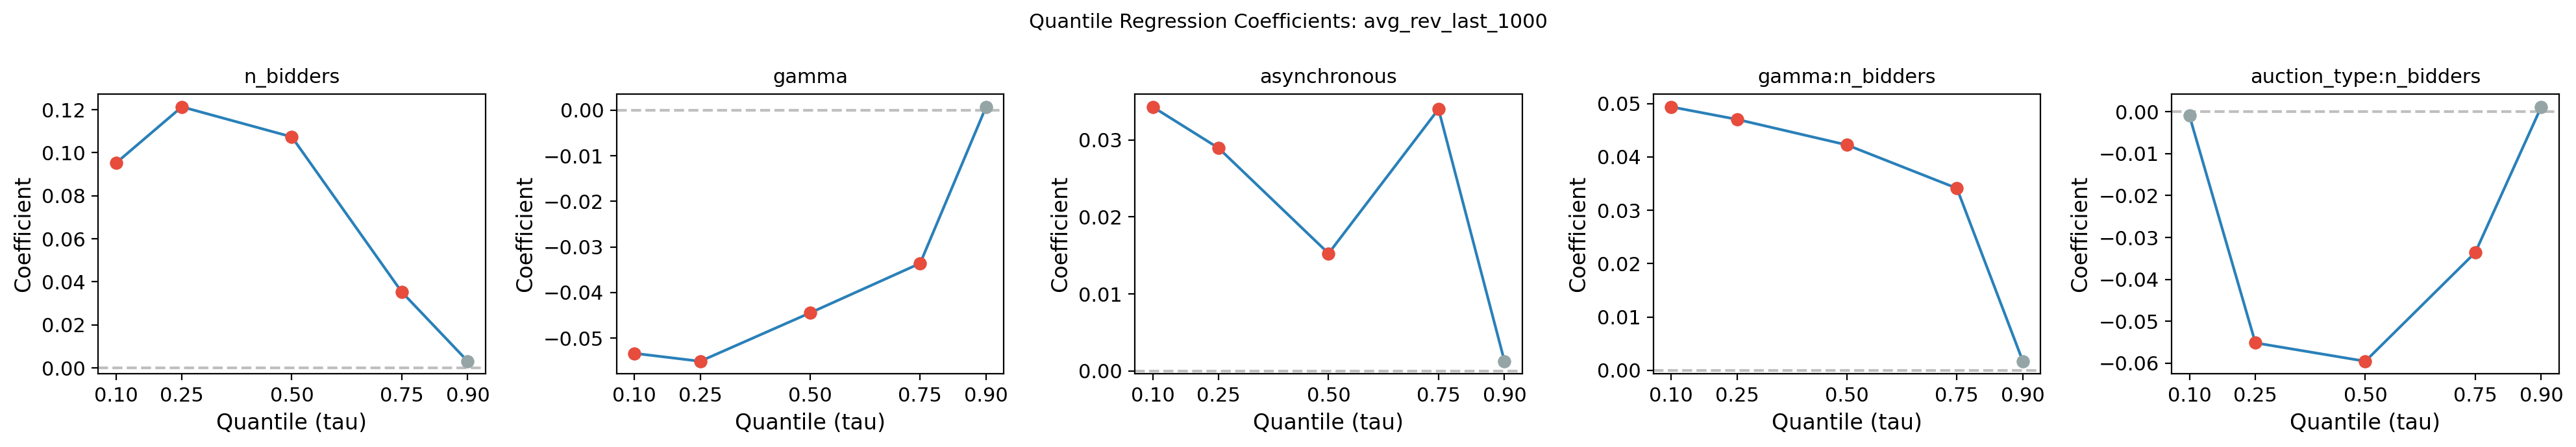
\includegraphics[width=0.7\textwidth]{figures/e1_quantile_rev}
  \caption{Experiment~1: Quantile regression coefficients for average revenue at the 10th, 25th, 50th, 75th, and 90th percentiles. The auction type penalty is moderately larger in the left tail.}
  \label{fig:e1_quantile_rev}
\end{figure}

\input{tables/exp1_significant}

\subsection{Experiment~2}
\label{sec:exp2_robustness}

\input{tables/exp2_model_fit}

\input{tables/exp2_adequacy}

Table~\ref{tab:exp2_adequacy} reports model adequacy. LightGBM cross-validated $R^2$ is comparable to OLS $R^2$, confirming that the linear model with two-way interactions is correctly specified for this design.

\input{tables/exp2_inference_robust}

Table~\ref{tab:exp2_inference} reports inference robustness. Holm--Bonferroni and Benjamini--Hochberg corrections retain the key effects involving affiliation and number of bidders. Quantile regression effects are broadly symmetric across the response distribution (Figure~\ref{fig:e2_quantile_rev}).

\begin{figure}[H]
  \centering
  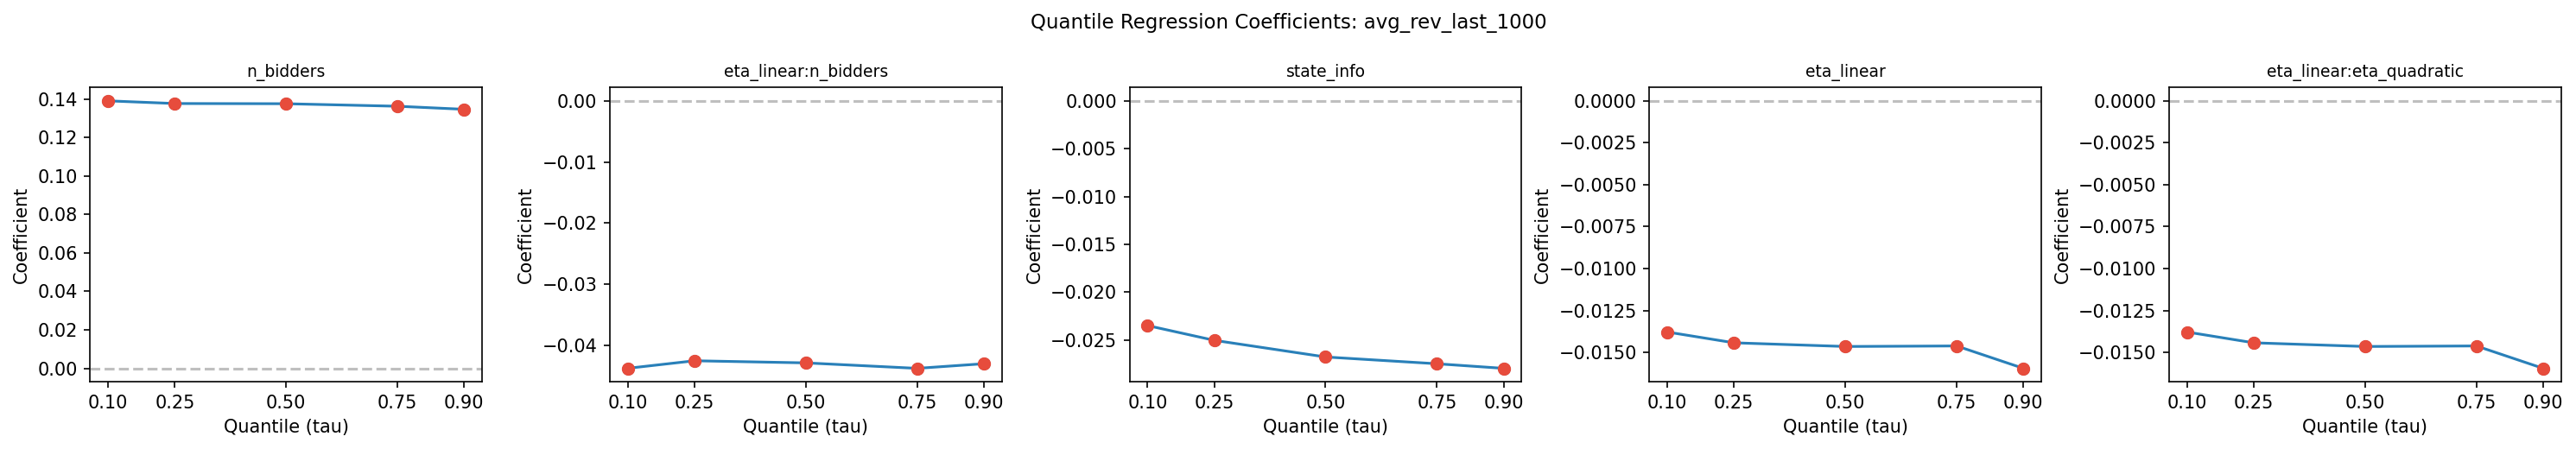
\includegraphics[width=0.7\textwidth]{figures/e2_quantile_rev}
  \caption{Experiment~2: Quantile regression coefficients for average revenue. The wide confidence bands reflect the limited replication of the $3 \times 2^3$ design.}
  \label{fig:e2_quantile_rev}
\end{figure}

\input{tables/exp2_significant}

\subsection{Experiment~3a (LinUCB)}
\label{sec:exp3a_robustness}

\input{tables/exp3a_model_fit}

\input{tables/exp3a_adequacy}

Table~\ref{tab:exp3a_adequacy} reports model adequacy for the LinUCB design. LightGBM cross-validated $R^2$ modestly exceeds OLS $R^2$ for revenue. The lack-of-fit test is significant for the primary responses, indicating detectable departures from the linear model with two-way interactions; however, the dominant factors (number of bidders, auction type) are robustly identified under both the linear and nonparametric models.

\input{tables/exp3a_inference_robust}

Table~\ref{tab:exp3a_inference} shows that Holm--Bonferroni and Benjamini--Hochberg corrections retain the key effects despite modest model misfit. Quantile regression reveals notable heterogeneity across the revenue distribution (Figure~\ref{fig:e3a_quantile_rev}): the auction type coefficient grows in magnitude from the lower to upper quantiles, indicating that first-price auctions disproportionately suppress revenue among the best-performing configurations.

\begin{figure}[H]
  \centering
  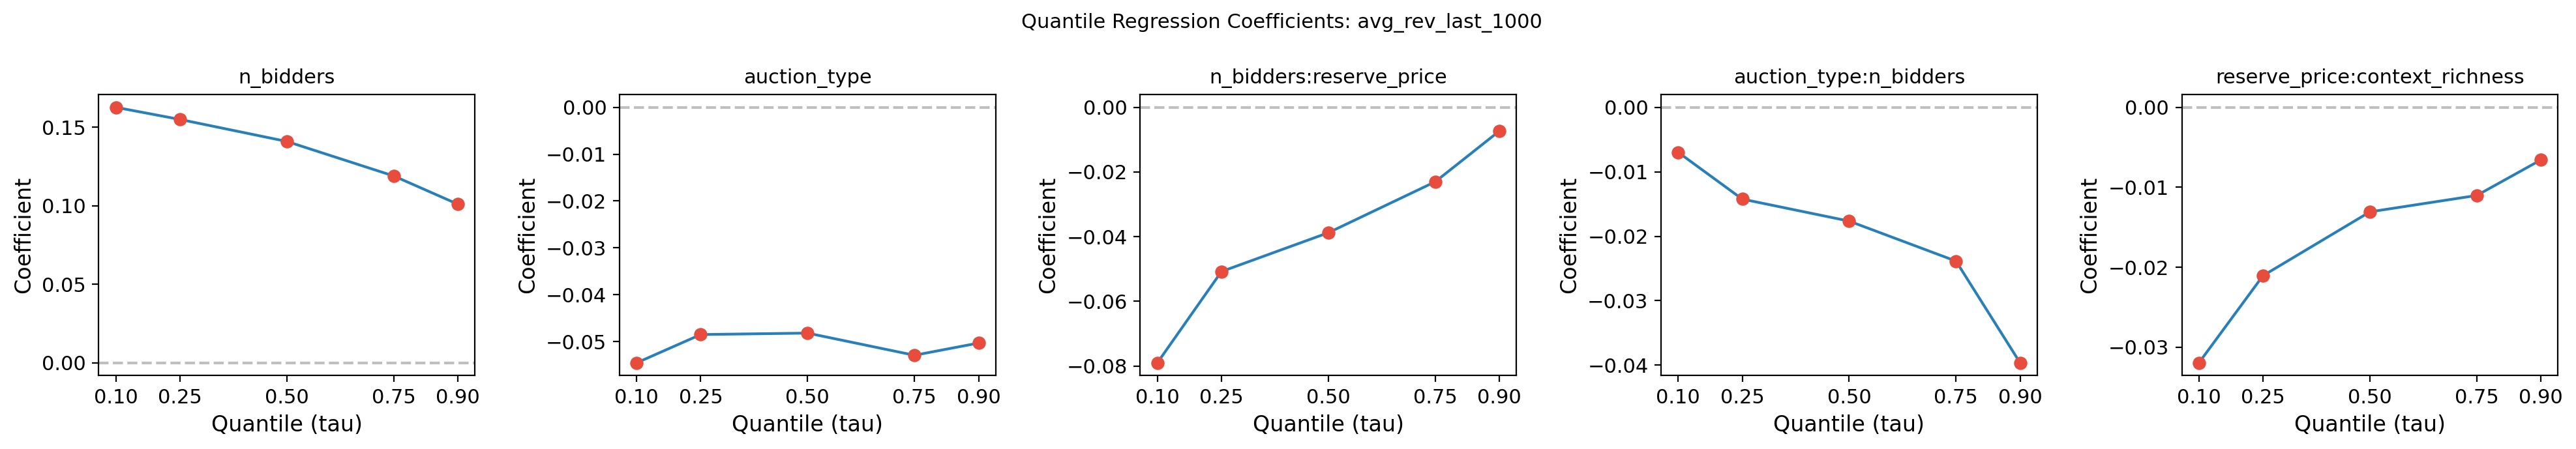
\includegraphics[width=0.7\textwidth]{figures/e3a_quantile_rev}
  \caption{Experiment~3a: Quantile regression coefficients for average revenue (LinUCB). The auction type penalty grows substantially from the 10th to the 90th percentile, indicating that the first-price disadvantage intensifies at higher revenue levels.}
  \label{fig:e3a_quantile_rev}
\end{figure}

\input{tables/exp3a_significant}

\subsection{Experiment~3b (Thompson Sampling)}
\label{sec:exp3b_robustness}

\input{tables/exp3b_model_fit}

\input{tables/exp3b_adequacy}

Table~\ref{tab:exp3b_adequacy} reports model adequacy for the Thompson Sampling design. LightGBM cross-validated $R^2$ and OLS $R^2$ are comparable, confirming that the linear model with two-way interactions is correctly specified.

\input{tables/exp3b_inference_robust}

Table~\ref{tab:exp3b_inference} shows that Holm--Bonferroni and Benjamini--Hochberg corrections retain the key effects. Quantile regression coefficients are broadly stable across the revenue distribution (Figure~\ref{fig:e3b_quantile_rev}).

\begin{figure}[H]
  \centering
  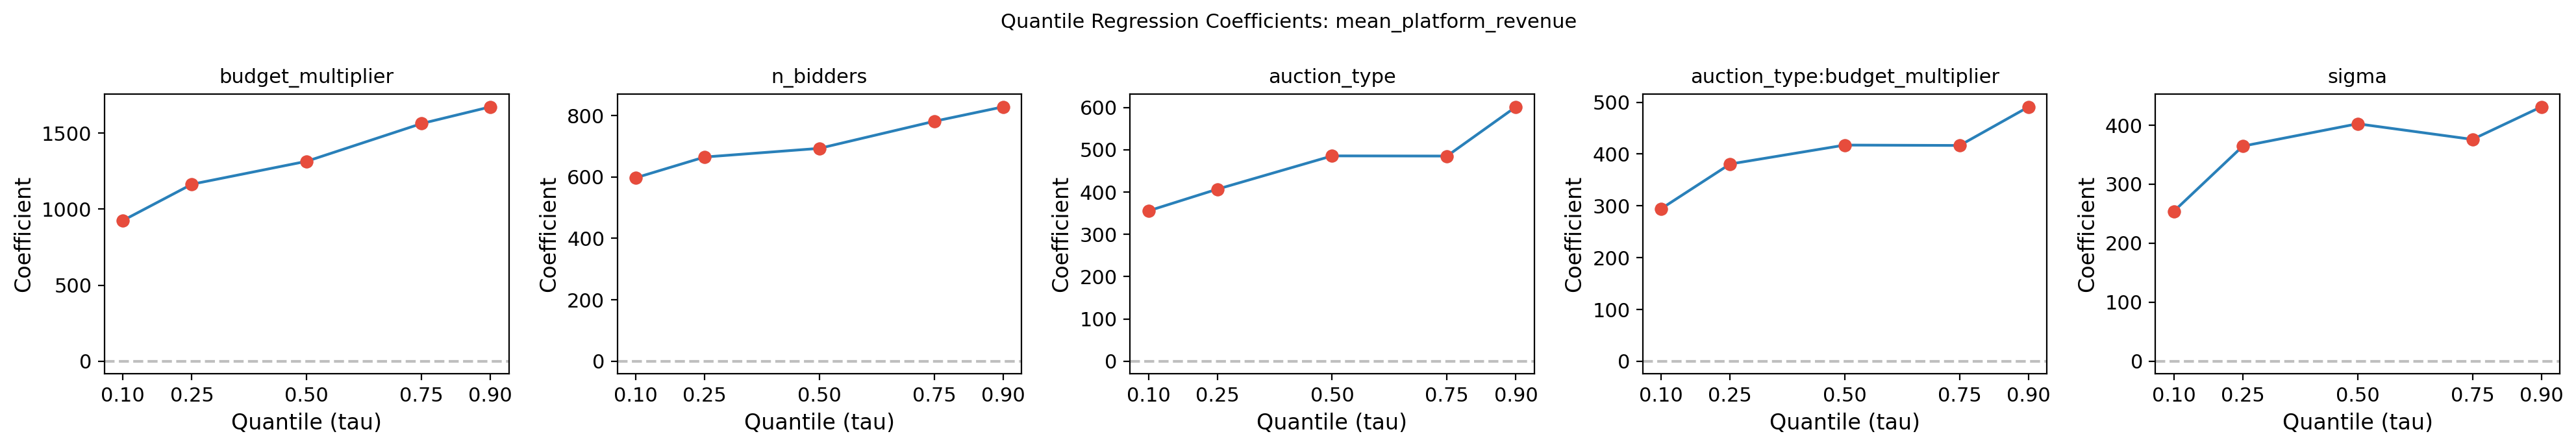
\includegraphics[width=0.7\textwidth]{figures/e3b_quantile_rev}
  \caption{Experiment~3b: Quantile regression coefficients for average revenue (Thompson Sampling).}
  \label{fig:e3b_quantile_rev}
\end{figure}

\input{tables/exp3b_significant}

\subsection{Experiment~4a}
\label{sec:exp4a_robustness}

\input{tables/exp4a_model_fit}

\input{tables/exp4a_adequacy}

Table~\ref{tab:exp4a_adequacy} reports model adequacy for the three primary responses. Platform revenue ($R^2 = 0.83$) and effective Price of Anarchy ($R^2 = 0.87$) show small PRESS gaps, indicating strong generalisability. The bid-to-value ratio achieves $R^2 = 0.99$. LightGBM cross-validated $R^2$ is substantially lower than OLS $R^2$ for all responses, confirming that the $2^6$ factorial with a linear model is the correct specification.

\input{tables/exp4a_inference_robust}

Table~\ref{tab:exp4a_inference} reports inference robustness. Quantile regression reveals moderate heterogeneity for platform revenue (Figure~\ref{fig:e4a_quantile_rev}): the objective coefficient grows from $-546$ at the 10th percentile to $-953$ at the 90th percentile, indicating that the revenue penalty from utility-maximizing objectives is concentrated among high-revenue configurations. The number of bidders effect remains stable across quantiles ($988$--$1{,}169$), confirming that market thickness benefits revenue uniformly.

\begin{figure}[H]
  \centering
  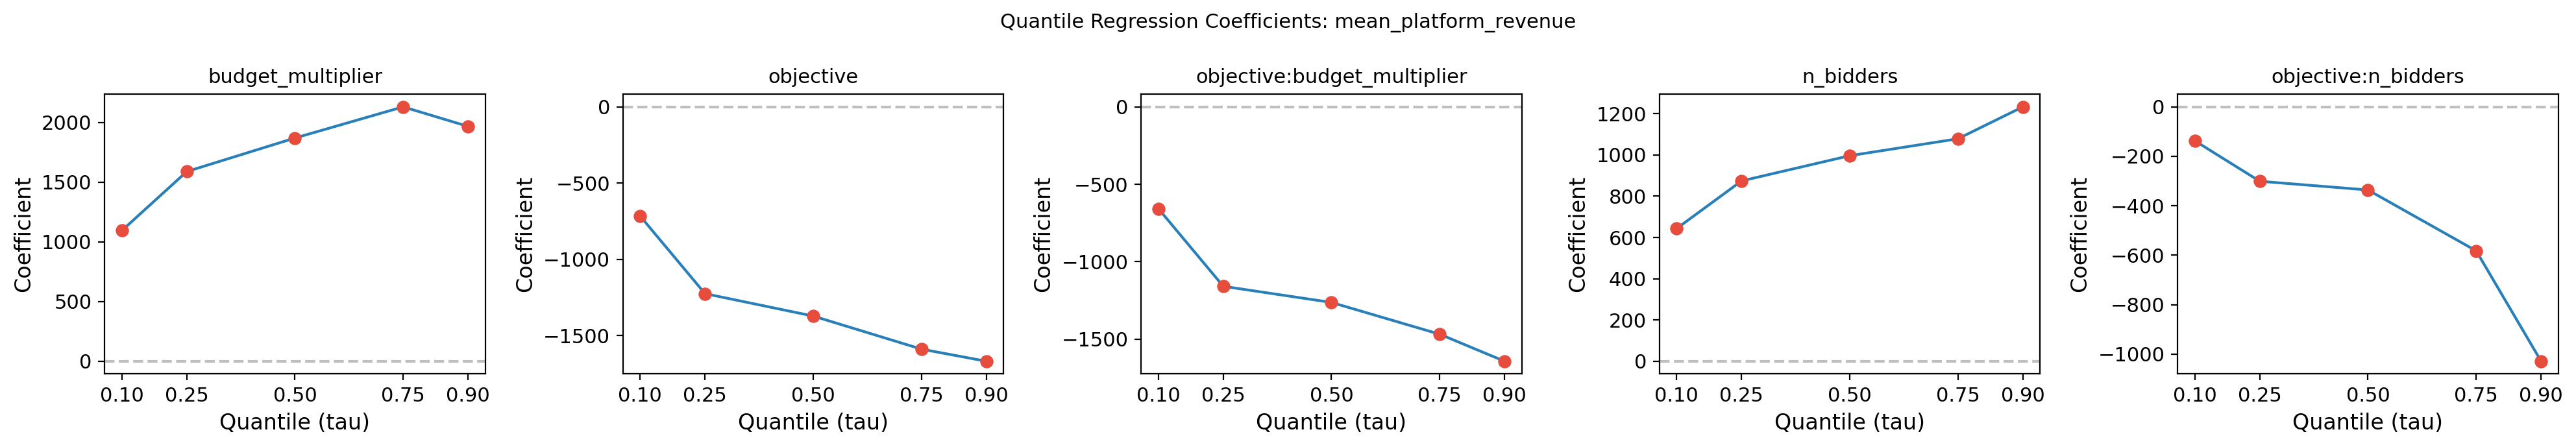
\includegraphics[width=0.7\textwidth]{figures/e4a_quantile_rev}
  \caption{Experiment~4a: Quantile regression coefficients for platform revenue. The objective effect (utility-maximiser vs.\ value-maximiser) grows substantially toward the upper tail.}
  \label{fig:e4a_quantile_rev}
\end{figure}

\input{tables/exp4a_significant}

\subsection{Experiment~4b}
\label{sec:exp4b_robustness}

\input{tables/exp4b_model_fit}

\input{tables/exp4b_adequacy}

Experiment~4b shares the $2^6$ factorial structure of Experiment~4a. Table~\ref{tab:exp4b_adequacy} reports model adequacy for the three primary responses. Platform revenue achieves $R^2 = 0.77$ with a PRESS gap of 0.022, comparable to Experiment~4a. The bid-to-value ratio is well-explained ($R^2 = 0.86$, gap 0.013), while effective Price of Anarchy has moderate explanatory power ($R^2 = 0.39$, gap 0.056). LightGBM cross-validated $R^2$ matches or falls below OLS for all responses, confirming that the linear factorial model captures the dominant variation.

\input{tables/exp4b_inference_robust}

\input{tables/exp4b_significant}

\subsection{Discretisation Sensitivity}
\label{sec:discretization_robust}

To verify that results are not driven by action space granularity, we re-run a representative subset of factorial cells at grid sizes of 6, 11, and 21 discrete bid levels for Experiments~1--3. Effect rankings are stable across grid sizes: the dominant factors (number of bidders, auction type) retain their relative ordering at all granularities. Mean response values shift modestly with grid size, consistent with the theoretical prediction that coarser grids introduce approximation error proportional to the grid spacing. Full results are available in \texttt{results/expN/robust/discretization/}.

\subsection{Budget Sensitivity (Experiment~4a)}
\label{sec:budget_robust}

We re-run Experiment~4a with budget multipliers $m \in \{0.25, 0.5, 1.0\}$, where $B_i = m \cdot \mathbb{E}[v_i] \cdot T$. The baseline ($m = 0.5$) produces moderately constrained budgets. Tighter budgets ($m = 0.25$) amplify the effect of bidder objective on revenue, while relaxed budgets ($m = 1.0$) reduce auction format effects as budget constraints become non-binding. The ranking of number of bidders as the dominant factor is preserved across all budget levels. Full results are reported in \texttt{results/exp4a/robust/budget/}.
